\documentclass{ximera}  
\title{Sinusoidal Signals}  
\begin{document}  
\begin{abstract}  
Review of Sinusoidal Signals
\end{abstract}  
\maketitle



Sinusoidal signals are important because in electrical engineering we use them to analyze and test circuit performance. All periodic signals can be represented with sinusoidal signals of different amplitudes and phases using the Fourier series. 

A typical sinusoidal signal is shown in Figure \ref{sinusoid}. On the y-axis is the instantaneous value of the sinusoidal voltage and on the x-axis is time. Instantaneous values of voltage change from -1V to 1V with time. Sinusoidal signals can be characterized by the following parameters: peak amplitude, peak-to-peak, average, RMS, period, time-delay, and phase. Peak amplitude, peak-to-peak, average and RMS values, are read on the y-axis in Figure \ref{sinusoid}, whereas period, time delay and phase are read on the x-axis.


\begin{enumerate}
\item Sinusoidal signals can be represented as a function of time, or a function of angle. In Figures \ref{sin}, \ref{sinMinus45T} the signals are shown as a function of time, whereas signals in Figure \ref{sinPh}, \ref{sinMinus45Ph} are shown as a function of angle. Take a few minutes to see how the graphs are the same and how are they different.
\item Peak amplitude is measured on the y-axis as the length from the average value of the signal (in this case zero) to the maximum value of the signal (in this case 1). For signal shown in Figure \ref{sinusoid}, peak  amplitude has a constant value of $V_p=1$. 
\item The instantaneous value of the sinusoidal signal varies from -1 to 1V. The peak amplitude is a constant and it does not vary with time. 
\item Peak-to-peak is measured from the minimum value of the function (in this case -1) to the maximum value of the function (in this case 1).  For signal shown in Figure \ref{sinusoid}, peak-to-peak voltage has a constant value of  $V_{pp}=2$.
\item RMS or root-mean-square is defined as $v_{rms}=\frac{1}{T} \sqrt{\int_0^T v(t)^2 dt}$. For signal shown in Figure \ref{sinusoid}, and other sinusoidal signals of this form,  $v_{rms}=\frac{V_p}{\sqrt{2}}=\frac{1}{\sqrt{2}}=0.707$. Root mean square value is important because it represents the equivalent amount of DC power.  
\item Average value $v_{ave1}=\frac{1}{T} \int_0^T v(t) dt$. For the signal shown in Figure \ref{sinusoid}, the average value is $V_{ave1}=0$ because the function has the same area under the function in the positive and negative cycle. 
\item Period is measured on the x-axis as the length of one full cycle of the sinusoidal signal. For signal shown in Figure \ref{sinusoid}, this value is $period=T$
\item Time delay represents the lag (or lead) of one function with respect to another. For example, in Figure \ref{sinusoid}, function $ \cos(\omega t - 90^o)$ is time-delayed for $\tau = \frac{T}{4}$ with respect to $\cos (\omega t)$. To find the time delay for a sinusoidal signal from its phase, we look at the way to represent the phase $90^o$ in terms of the product of frequency and time. Since in the sinusoidal signal expression $\cos (\omega t + \Theta)$  phase $\Theta$ is added to $\omega t$ term, the phase has the same units as $\omega t$, and can be represented as the product of $\omega \tau = \theta$, $\tau = \frac{\theta}{\omega}$, where $\tau$ represents the time delay.
\item Different phases of the signal are shown in Figure \ref{sinMinus45T}-\ref{sinPlus45Ph}. 
\begin{enumerate}
\item When the phase of a signal is positive as in Figure \ref{sinPlus45Ph} $ \sin (\omega t + 45^o)$, we say that the signal is leading with respect to the signal $ \sin (\omega t)$, because it is shifted to the left for $45^o$($pi/4$), or $\tau=+\frac{pi/4}{\omega} $. The leading function's peak occurs earlier in time, and therefore it is leading. The phase of the signal is $45^o$. 
\item When the phase of a signal is negative as in Figure \ref{sinMinus45T}, \ref{sinMinus45Ph} $ \sin (\omega t - 45^o)$, we say that the signal is lagging with respect to the signal $ \sin (\omega t)$, because it is shifted to the right for $45^o$ ($pi/4$), or $\tau=-\frac{pi/4}{\omega} $. The lagging function's peak occurs later in time, and therefore it is lagging. The phase of the signal is $-45^o$.
\end{enumerate}
\end{enumerate}


\begin{figure}
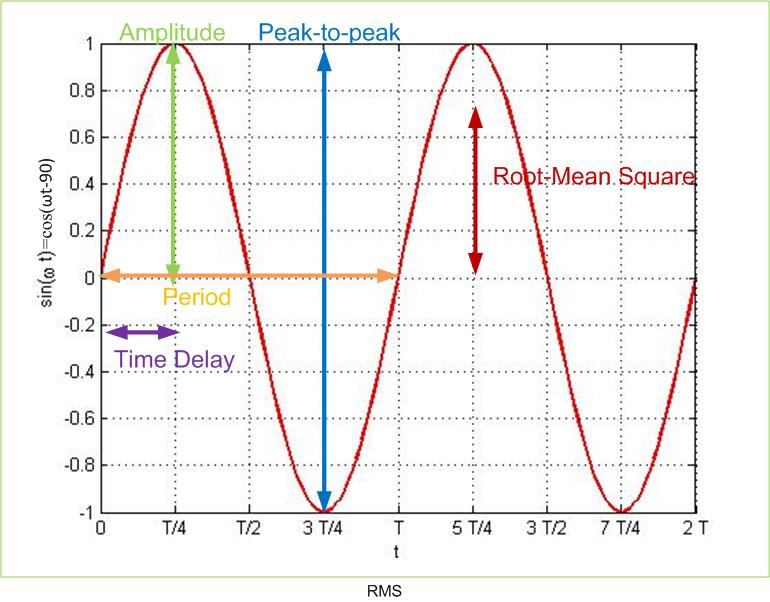
\includegraphics{jpg/sinusoid.jpg}
\caption{Vocabulary used in describing sinusoidal signals.}
\label{sinusoid}
\end{figure} 





\begin{figure}
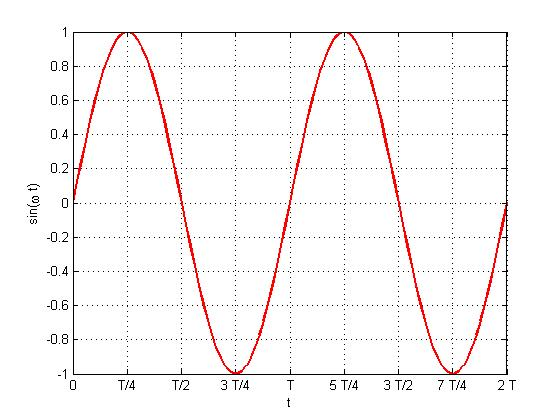
\includegraphics{jpg/cpef1.jpg}
\caption{$sin ( \omega t)$ as a function of time.} \label{sin}
\end{figure}


\begin{figure}
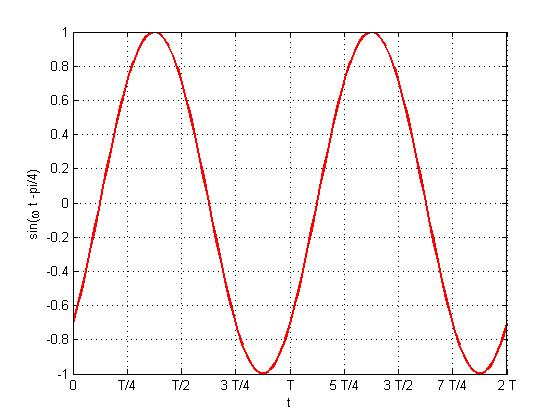
\includegraphics{jpg/cpef2.jpg}
\caption{ Sinusoidal signal shifted for time delay $-\frac{\pi/4}{\omega}$}
\label{sinMinus45T}
\end{figure}

\begin{figure}
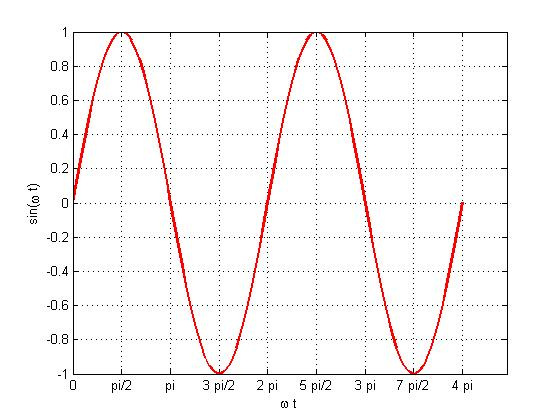
\includegraphics{jpg/cpef3.jpg}
\caption{Sinusoidal signal as a function of angle $\omega t$.}
\label{sinPh}
\end{figure}

\begin{figure}
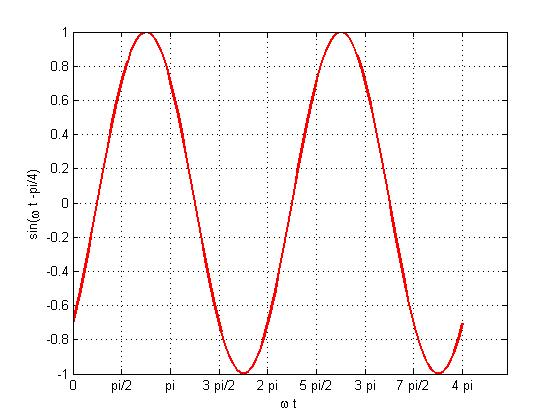
\includegraphics{jpg/cpef4.jpg}
\caption{Sinusoidal signal as a function of angle $\omega t$ with a phase shift of $-\pi/4$}
\label{sinMinus45Ph}
\end{figure}

\begin{figure}
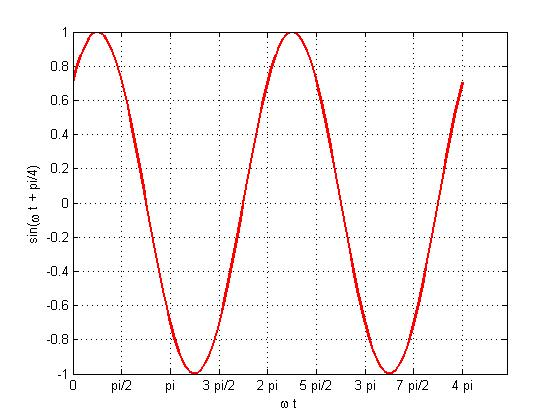
\includegraphics{jpg/cpef5.jpg}
\caption{Sinusoidal signal as a function of angle $\omega t$ with a phase shift of $+\pi/4$}
\label{sinPlus45Ph}
\end{figure}



\begin{figure}
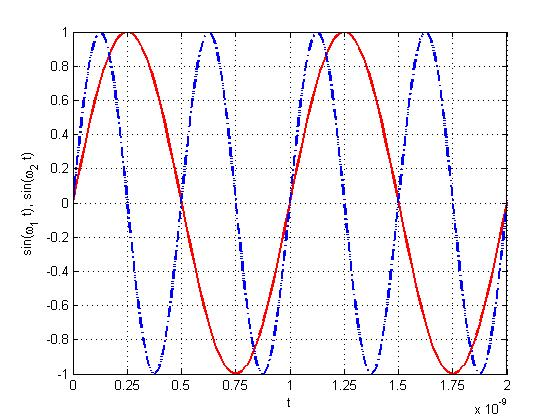
\includegraphics[scale=0.4]{jpg/cpef6.jpg}
\caption{Sinusoidal signals of different frequencies $sin ( \omega t)$}
\label{sinF1F2}
\end{figure}


%\begin{image}
%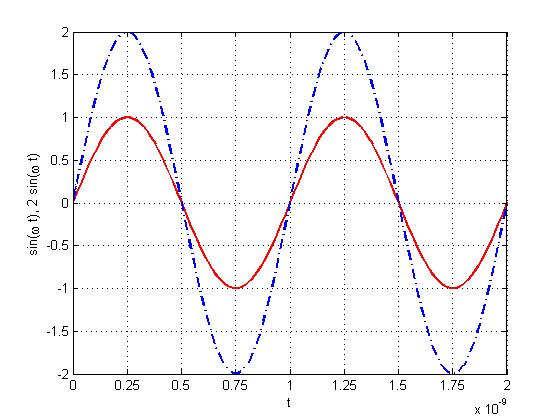
\includegraphics[scale=0.4]{jpg/cpef7.jpg}
%\caption{Sinusoidal signals of different amplitudes $sin ( \omega t)$}\label{sinA1A2}
%\end{image}


\begin{image}
\begin{tikzpicture}
    \begin{axis}[
            xmin=-1.1,xmax=1.1,ymin=-1.1,ymax=1.1,
            axis lines=center,
            width=4in,
            xtick={-1,1},
            ytick={-1,1},
            clip=false,
            unit vector ratio*=1 1 1,
            xlabel=$x$, ylabel=$y$,
            every axis y label/.style={at=(current axis.above origin),anchor=south},
            every axis x label/.style={at=(current axis.right of origin),anchor=west},
          ]        
          \addplot [dashed, smooth, domain=(0:360)] ({cos(x)},{sin(x)}); %% unit circle

          \addplot [textColor] plot coordinates {(0,0) (.766,.643)}; %% 40 degrees

          \addplot [ultra thick,penColor] plot coordinates {(.766,0) (.766,.643)}; %% 40 degrees
          \addplot [ultra thick,penColor2] plot coordinates {(0,0) (.766,0)}; %% 40 degrees
          
          %\addplot [ultra thick,penColor3] plot coordinates {(1,0) (1,.839)}; %% 40 degrees          

          \addplot [textColor,smooth, domain=(0:40)] ({.15*cos(x)},{.15*sin(x)});
          %\addplot [very thick,penColor] plot coordinates {(0,0) (.766,.643)}; %% sector
          %\addplot [very thick,penColor] plot coordinates {(0,0) (1,0)}; %% sector
          %\addplot [very thick, penColor, smooth, domain=(0:40)] ({cos(x)},{sin(x)}); %% sector
          \node at (axis cs:.15,.07) [anchor=west] {$\theta$};
          \node[penColor, rotate=-90] at (axis cs:.84,.322) {$\sin(\theta)$};
          \node[penColor2] at (axis cs:.383,0) [anchor=north] {$\cos(\theta)$};
          %\node[penColor3, rotate=-90] at (axis cs:1.06,.322) {$\tan(\theta)$};
        \end{axis}
\end{tikzpicture}
\caption{Unit Circle} \label{unitCircle}
\end{image}



\begin{image}
\begin{tikzpicture}
    \begin{axis}[
            xmin=-6.75,xmax=6.75,ymin=-1.5,ymax=1.5,
            axis lines=center,
            xtick={-6.28, -4.71, -3.14, -1.57, 0, 1.57, 3.142, 4.71, 6.28},
            xticklabels={$-2\pi$,$-3\pi/2$,$-\pi$, $-\pi/2$, $0$, $\pi/2$, $\pi$, $3\pi/2$, $2\pi$},
            ytick={-1,1},
            %ticks=none,
            width=6in,
            height=3in,
            unit vector ratio*=1 1 1,
            xlabel=$\theta$, ylabel=$x$,
            every axis y label/.style={at=(current axis.above origin),anchor=south},
            every axis x label/.style={at=(current axis.right of origin),anchor=west},
          ]        
          \addplot [very thick, penColor, samples=100,smooth, domain=(-6.75:6.75)] {cos(deg(x))};
        \addplot [very thick, penColor4, samples=100,smooth, domain=(-6.75:6.75)] {cos(deg(x)+90)};
         \addplot [very thick, penColor2, samples=100,smooth, domain=(-6.75:6.75)] {cos(deg(x)-90)};
                   
          \node at (axis cs:-3,-1.2) [penColor] {$\cos(\theta)$};
          \node at (axis cs:-1.72, 1.2) [penColor4] {$\cos(\theta + \pi/4)$};
        \node at (axis cs:3, 1.2) [penColor2] {$\cos(\theta - \pi/4)$};
        \end{axis}
\end{tikzpicture}
%% \caption{The function $\cos(\theta)$ takes on all values between $-1$
%%   and $1$ exactly once on the interval $[0,\pi]$. If we restrict
%%   $\cos(\theta)$ to this interval, then this restricted function has
%%   an inverse.}
%% \label{figure:cos-restricted}
%% \end{figure*}
\caption{$\cos (\omega t)$}\label{cosine}
\end{image}







                                                                   



                                       




                                    














\end{document}



                                                                   



                                       




                                    














\maketitle    
  Calculate.
\begin{question}  
$3\times 2 = \answer{6}$  
\end{question} 
\end{document} 
